\chapter{Bound States in the Continuum and Exceptional Topology}
\label{ch:bic-topology}

\begin{chapterlead}
Not all non-Hermitian phenomena involve complex eigenfrequencies. A
\emph{bound state in the continuum} (BIC)~\cite{hsu2016bound,koshelev2018nonradiating,kang2023applications,koshelev2018asymmetric,kang2022merging,bai2024recovery,gao2024degenerate} is a mode with a real
eigenfrequency embedded within the radiation continuum---a state that,
by symmetry or fine-tuning, is perfectly decoupled from all outgoing
channels despite coexisting spectrally with radiation modes. BICs often
behave as topological objects: in photonic crystal slabs with a
well-defined far-field polarization, they carry quantized charges in
momentum space and can be connected to exceptional points through the
analytic structure of open-system resonances. The BIC condition is
derived from the Maxwell problem, the role of topological charge is
identified, and photonic crystal slabs serve as the main examples.
\end{chapterlead}


%% ================================================================
\section{What is a bound state in the continuum?}
\label{sec:bic-definition}

In an open photonic structure---a photonic crystal slab, a grating, or
a metasurface---most resonances are quasinormal modes with complex
frequencies $\omtil = \omega - i\gamma$ and finite quality factors
(Chapter~\ref{ch:qnm}). A BIC is the exception: it has $\gamma = 0$
(infinite $\Qfac$) despite lying within the frequency range where
radiation channels are open.

Formally, a BIC is a normalizable solution of the source-free Maxwell
equations at a real frequency $\omega_{\mathrm{BIC}}$ that satisfies
$\omega_{\mathrm{BIC}} > \omega_{\mathrm{light\;line}}$---above the
light line, where radiation modes exist---yet has zero coupling to all
radiation channels.

\subsection{The radiation-amplitude viewpoint}
\label{ssec:radiation-amplitude}

To make the BIC condition precise within the Maxwell framework, consider
a photonic crystal slab of thickness $d$ with in-plane periodicity. At
each Bloch wave vector $\kk_\parallel$ and frequency $\omega$, the
far-field radiation above and below the slab can be decomposed into a
finite number of open diffraction channels, each carrying a transverse
polarization. Let $c_j(\kk_\parallel)$ denote the complex amplitude
radiated into channel $j$. The total radiation rate is
\begin{equation}
 \gamma(\kk_\parallel) \propto \sum_j |c_j(\kk_\parallel)|^2.
 \label{eq:radiation-rate}
\end{equation}
A BIC occurs when every \emph{open} radiation amplitude vanishes
simultaneously:
\begin{equation}
 c_j(\kk_{\mathrm{BIC}}) = 0 \quad \text{for all open channels } j.
 \label{eq:bic-all-zero}
\end{equation}
This is a set of conditions---one complex equation per independent
channel amplitude, modulo symmetry and phase constraints---so generic
BICs normally require tuning. At high-symmetry points where symmetry
forbids certain channels, fewer conditions remain and BICs arise more
naturally.

\subsection{Symmetry-protected BICs}
\label{ssec:symmetry-bic}

A symmetry-protected BIC exists at high-symmetry points in the Brillouin
zone (e.g., $\Gamma$) where the mode belongs to an irreducible
representation that is incompatible with the radiation continuum. For
example, a mode that is odd under a $C_2$ rotation of the slab cannot
couple to normally incident plane waves, which transform as the trivial
representation. The decoupling is exact and persists under any
perturbation that preserves the symmetry.

At the $\Gamma$ point of a square-lattice photonic crystal slab, the
point group is $C_{4v}$. Modes belonging to the $B_1$ or $B_2$
representations are incompatible with the $s$- and $p$-polarized plane
waves (which belong to $A_1$ and $E$), ensuring zero radiation. Moving
away from $\Gamma$ reduces the symmetry, and the mode acquires a finite
radiation rate---becoming a quasi-BIC with high but finite $\Qfac$.

\subsection{Accidental (tuned) BICs}
\label{ssec:accidental-bic}

At generic $\kk$-points away from high-symmetry positions, BICs can
arise from a destructive interference between two or more radiation
channels. These accidental BICs require fine-tuning of one structural
parameter (e.g., the slab thickness, hole radius, or lattice constant)
and are generically isolated points in the $(\kk, \text{parameter})$
space.

Near an accidental BIC, the radiation amplitudes vanish linearly:
$c_j \propto |\kk - \kk_{\mathrm{BIC}}|$. Since $\gamma \propto
\sum |c_j|^2$, the quality factor diverges as
\begin{equation}
 \Qfac(\kk) \propto \frac{1}{|\kk - \kk_{\mathrm{BIC}}|^2},
 \label{eq:bic-Q-divergence}
\end{equation}
producing a family of ultra-high-$\Qfac$ quasi-BIC resonances in the
vicinity.
\begin{figure}[t]
 \centering
 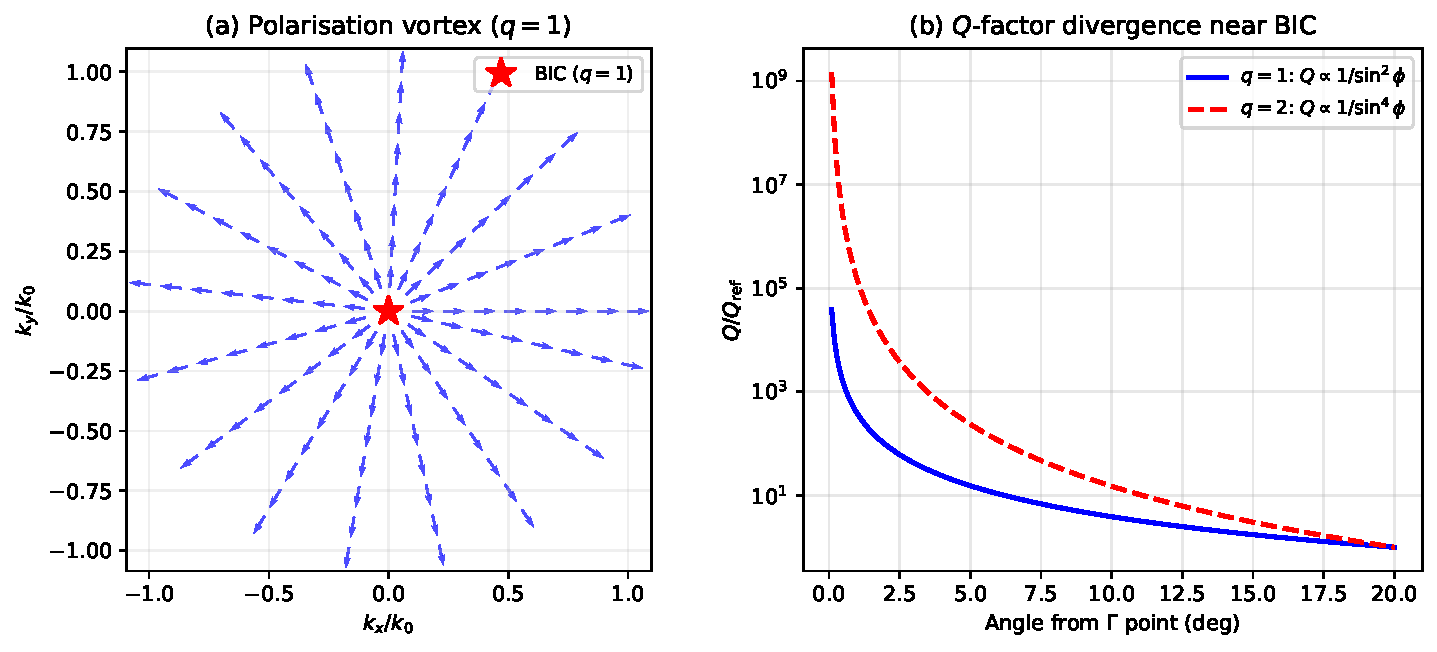
\includegraphics[width=0.85\linewidth]{figures/fig_f16_bic_farfield.pdf}
 \caption{Far-field polarization vortex and quality-factor divergence
 near a symmetry-protected BIC. (a)~The polarization direction winds
 once around the BIC in momentum space, giving topological charge
 $q=1$. (b)~The radiative quality factor diverges as the far-field
 radiation amplitude vanishes; higher-charge vortices produce steeper
 $Q$-scaling. This figure connects the Maxwell radiation amplitudes
 $c_j(\kk)$ in Eq.~\eqref{eq:radiation-rate} to the polarization
 topology used to classify BICs.}
 \label{fig:bic-farfield-vortex}
\end{figure}


\subsection{Other BIC mechanisms}
\label{ssec:other-bic}

Beyond symmetry protection and parametric tuning, BICs can also arise
through Fabry--P\'erot interference (standing waves in the slab thickness
direction that decouple from radiation), Friedrich--Wintgen avoided
crossing (two resonances exchanging their radiation channels so that one
becomes dark), and inverse-construction methods that engineer the
potential or hopping rates to produce a bound state at a desired
location~\cite{wang2023brillouin}. The common thread is the vanishing
of all radiation amplitudes~\eqref{eq:bic-all-zero}.

\subsection{Friedrich--Wintgen avoided crossing}
\label{ssec:friedrich-wintgen}

A particularly instructive BIC mechanism arises from the avoided crossing
of two resonances coupled through a shared radiation continuum. Consider
two quasi-bound modes $|1\rangle$ and $|2\rangle$ with complex frequencies
$\omtil_j = \omega_j - i\gamma_j$ that approach each other as a structural
parameter is varied. In the two-mode TCMT of
Chapter~\ref{ch:maxwell-coupled-modes}, the effective Hamiltonian including
radiation coupling is
\begin{equation}
 H_{\mathrm{FW}} =
 \begin{pmatrix}
 \omega_1 - i\gamma_1 & \kappa - i\sqrt{\gamma_1\gamma_2}\,e^{i\phi} \\
 \kappa - i\sqrt{\gamma_1\gamma_2}\,e^{-i\phi} & \omega_2 - i\gamma_2
 \end{pmatrix},
 \label{eq:fw-hamiltonian}
\end{equation}
where $\kappa$ is the near-field coupling and the off-diagonal imaginary
term represents far-field coupling mediated by the shared continuum, with
relative phase $\phi$. Friedrich and Wintgen showed that there exists a
parameter value at which one eigenvalue becomes purely real: the radiation
widths of the two modes rearrange so that one mode absorbs all the
radiation and the other becomes a BIC with $\gamma = 0$.

In this two-mode model the Friedrich--Wintgen BIC occurs when the dark
eigenvector is orthogonal to the continuum-coupling vector. For the
phase convention of Eq.~\eqref{eq:fw-hamiltonian}, this can be written
schematically as
\begin{equation}
 \frac{\kappa}{\sqrt{\gamma_1\gamma_2}} = \frac{\omega_1 - \omega_2}{\gamma_1 - \gamma_2}\,\sin\phi,
 \label{eq:fw-condition}
\end{equation}
with the precise form depending on the normalization of the radiative
coupling amplitudes. The essential requirement is destructive
interference of the two radiative pathways, which can be satisfied by
tuning $\omega_1-\omega_2$ through a structural parameter. This mechanism
is responsible for many accidental BICs observed in photonic crystal slabs: two modes of different symmetry
character exchange their radiation through the continuum, and at one
particular geometry one mode becomes perfectly dark while the other
becomes superradiant. The BIC produced by this mechanism carries a
topological charge $|q| = 1$, consistent with the general framework~\cite{zhen2014topological,zhen2015spawning,plotnik2011experimental,mohamed2020topological} of
Section~\ref{sec:bic-charge}.
\begin{figure}[t]
 \centering
 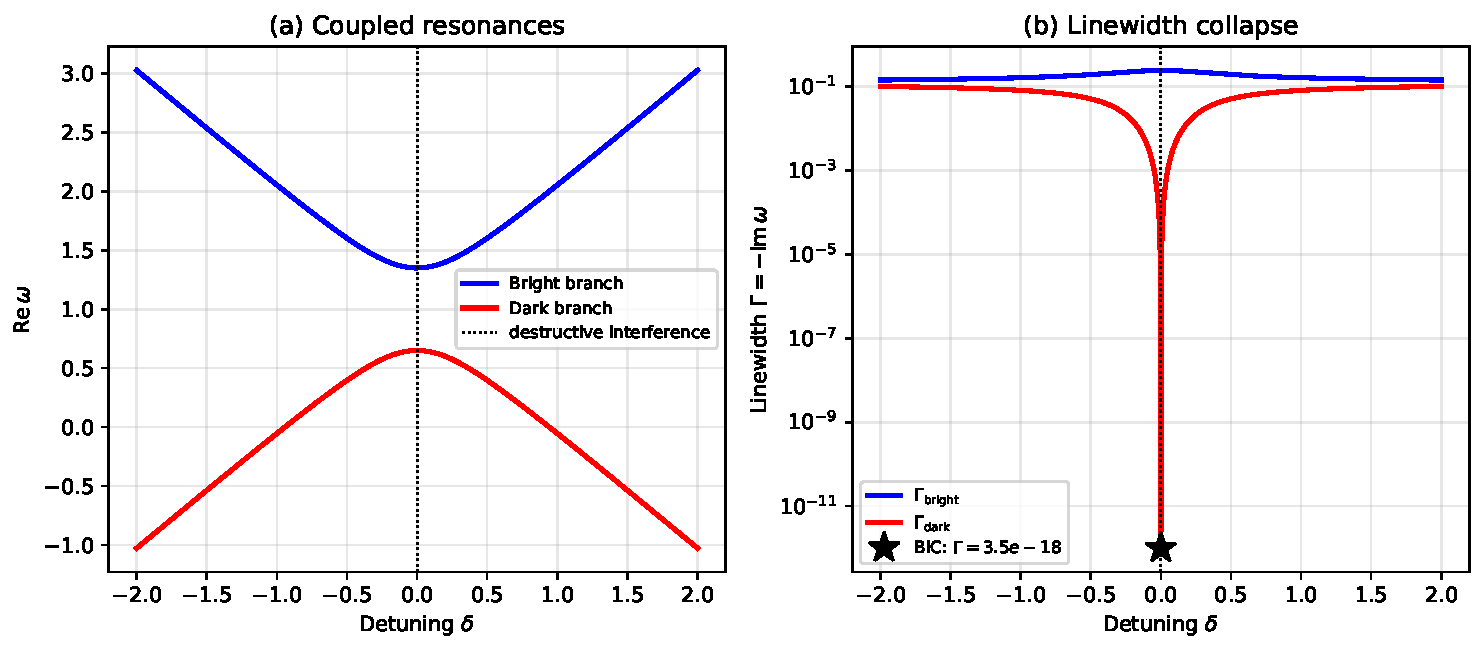
\includegraphics[width=0.85\linewidth]{figures/fig_f16_friedrich_wintgen.pdf}
 \caption{Friedrich--Wintgen BIC from destructive interference in a
 shared radiation channel. (a)~Two coupled resonances exchange their
 bright and dark character as a detuning parameter is swept.
 (b)~The dark branch linewidth collapses at $\delta=0$; the numerical
 model gives a linewidth limited by numerical precision away from scan
 boundaries, consistent with a genuine BIC rather than a finite-$Q$ minimum.
 The bright branch becomes superradiant, carrying the radiative loss
 removed from the dark state.}
 \label{fig:friedrich-wintgen-linewidth}
\end{figure}



%% ================================================================
\section{Topological charge of a BIC}
\label{sec:bic-charge}

Many BICs in photonic crystal slabs are \emph{topological objects}: when the relevant far-field
radiation can be represented by a continuous two-component polarization
field, each radiation zero carries a quantized charge defined by the
winding of that field around the BIC in momentum space~\cite{doeleman2018experimental,wang2020generating,liu2021topological,kang2023applications,yoda2020generation,qin2023arbitrarily}.

\subsection{Far-field polarization as a vector field on the BZ}
\label{ssec:farfield-polarization}

For a photonic crystal slab, each resonance at $\kk_\parallel$ radiates
into the zeroth diffraction order with a well-defined polarization
state. In the far field, this polarization can be represented by a
Jones vector $(E_x, E_y)$ or, equivalently, by the angle $\theta(\kk)$
of the major axis of the polarization ellipse. As $\kk$ varies over
the Brillouin zone, $\theta(\kk)$ defines a continuous (except at
singular points) direction field on the 2D momentum
plane~\cite{wang2023brillouin}.

At a BIC, the radiation amplitude vanishes---the polarization becomes
undefined. The BIC is a \emph{singularity} of the polarization field,
analogous to a vortex core in a fluid or a topological defect in a
liquid crystal.

\subsection{The charge integral}
\label{ssec:charge-integral}

Around a BIC at $\kk_{\mathrm{BIC}}$, the far-field angle $\theta$
can wind by an integer multiple of $2\pi$ when a real polarization
vector convention is available:
\begin{equation}
 \boxed{
 q = \frac{1}{2\pi}\oint_{\mathcal{C}}
 \dd\theta(\kk) \;\in\; \mathbb{Z},
 }
 \label{eq:bic-topological-charge}
\end{equation}
where $\mathcal{C}$ is a small closed loop enclosing $\kk_{\mathrm{BIC}}$.
The integer $q$ is the \emph{topological charge} of the BIC.

A charge $q = +1$ corresponds to a counterclockwise $2\pi$ winding of
the far-field polarization vector; $q = -1$ to a clockwise winding.
If only an ellipse major axis is used, the director nature of the angle
must be treated carefully because $\theta$ and $\theta+\pi$ describe the
same axis. Higher-order charges $|q| > 1$ are possible but require
additional symmetry or fine-tuning.

\begin{figure}[t]
 \centering
 
\includegraphics[width=0.95\textwidth]{fig_f16_bic_polarization_charge.pdf}
 \caption{A BIC is a singularity of the far-field polarization vector. The arrows show a pedagogical polarization direction field around two radiation zeros: a charge-$+1$ BIC and a charge-$-1$ BIC. The dashed loop is the contour $\mathcal{C}$ in the charge integral~\eqref{eq:bic-topological-charge}.}
 \label{fig:bic-polarization-charge}
\end{figure}


\begin{booknote}[Why the charge is topological]
The integral~\eqref{eq:bic-topological-charge} is a topological invariant
because $\theta(\kk)$ is continuous everywhere on $\mathcal{C}$ (the
loop does not pass through a BIC), and the total winding is insensitive
to smooth deformations of the loop. A small perturbation of the
photonic structure changes $\theta(\kk)$ continuously but cannot change
the integer $q$ unless the BIC moves through the loop or another
singularity enters or leaves.
\end{booknote}

\subsection{Charge conservation and annihilation}
\label{ssec:charge-conservation}

Topological charges are conserved under smooth structural perturbations.
This conservation law follows directly from the continuity of the
radiation amplitudes $c_j(\kk_\parallel)$ as functions of both
momentum and structural parameters.

To prove conservation, note that the topological charge $q$ of a BIC is
defined as the winding number of the polarization angle $\theta(\kk)$
on a closed loop $\mathcal{C}$ encircling the BIC in momentum space.
As a structural parameter $\alpha$ (such as the hole radius or slab
thickness) is varied smoothly, the radiation amplitudes
$c_j(\kk; \alpha)$ change continuously. The BIC position
$\kk_{\mathrm{BIC}}(\alpha)$ traces a smooth curve in the Brillouin
zone, and as long as the loop $\mathcal{C}$ does not cross another BIC,
the winding number cannot change---it is a topological invariant of the
loop. This is the photonic analogue of the conservation of vortex
charge in superfluid dynamics: a quantized topological object cannot be
created or destroyed by smooth deformations.

A BIC can only disappear through \emph{annihilation} with another BIC
of opposite charge. When two BICs with charges $q_1$ and $q_2$ are
brought together by tuning $\alpha$, the radiation amplitudes on a loop
encircling both BICs have total winding $q_1 + q_2$. If
$q_1 + q_2 = 0$, the net winding vanishes, and the merged state is no
longer topologically protected: both modes become leaky with finite
$\Qfac$. The annihilation is a codimension-one event in parameter
space---it requires tuning a single parameter to bring the BICs into
coincidence---and the quality factor drops abruptly from infinity to a
finite value at the annihilation point.

Conversely, if $q_1 + q_2 \neq 0$, the merged state retains a nonzero
charge $|q_{\mathrm{merged}}| = |q_1 + q_2|$ and remains a BIC. This
is the \emph{charge addition} rule that underlies the super-BIC
construction of Section~\ref{sec:bic-merging}. The radiation rate near
the merged BIC is suppressed as
$\gamma(\kk) \propto |\kk - \kk_{\mathrm{BIC}}|^{2|q_{\mathrm{merged}}|}$,
which scales more steeply than either parent BIC. The charge addition
rule is summarised by the algebra
\begin{equation}
 q_{\mathrm{merged}} = q_1 + q_2, \qquad
   \gamma \propto |\Delta k|^{2|q_1 + q_2|}, \qquad
 \Qfac_{\mathrm{finite}} \propto N^{2|q_1 + q_2|},
 \label{eq:charge-algebra}
\end{equation}
where $N$ is the number of periods in a finite structure and the
scaling assumes that the dominant radiation contribution comes from
Bloch components within $\Delta k \sim 1/N$ of the BIC, so that
$\gamma_{\mathrm{finite}} \propto (1/N)^{2|q|}$.  The assumption holds
for structures large enough that edge diffraction is subdominant.  Under
this condition, the formula is the central quantitative prediction of
the topological charge framework: it directly links the momentum-space
topology of the far field to the experimentally measurable $Q$-factor
scaling.

The creation--annihilation mechanism is directly analogous to the
pair creation and annihilation of Dirac cones in graphene-like
systems~\cite{guinea2009energy}, where merging two Dirac points of
opposite Berry phase ($\pm\pi$) opens a gap, while merging two points
of the same phase preserves the topological protection. In the BIC
context, the ``gap opening'' corresponds to the onset of radiative loss.

\paragraph{Connection to exceptional topology.}
The charge conservation of BICs is related, in specific models, to the
exceptional topology of Chapter~\ref{ch:exceptional-points}. When a BIC
is perturbed into a quasi-BIC, the relevant complex eigenfrequency
surface $\omtil(\kk,\alpha)$ can develop EPs in the extended parameter
space. In such cases the BIC may be viewed as a real-frequency radiation
zero that constrains how nearby eigenvalue sheets branch. The
topological charge of the BIC is then related to, but not generally
identical with, the discriminant number of the nearby EP. A rigorous
identification requires that the radiation channels and the eigenvalue
sheets share the same branch structure. This link has been demonstrated
for specific slab geometries by tracking BIC and EP positions as a
structural parameter is varied~\cite{zhen2015spawning}, but it is not a
model-independent theorem.

\subsection{Charge assignment in photonic crystal slabs}
\label{ssec:charge-assignment}

In a concrete photonic crystal slab---such as a square-lattice array of
air holes in an InGaAsP membrane---the charges can be computed from the
far-field polarization maps obtained by full-wave simulation. A
symmetry-protected BIC at the $\Gamma$ point typically carries charge
$q = +1$, while accidental BICs along high-symmetry directions carry
$q = \pm 1$ depending on their position in the Brillouin zone.
In the simulations of
Hwang et al., the symmetry-protected BIC at $\Gamma$ has $q = +1$, four
accidental BICs on the $\Gamma$--$M$ lines have $q = +1$, and four
accidental BICs on the $\Gamma$--$X$ lines have $q = -1$, giving a total
charge of $1 + 4(+1) + 4(-1) = +1$ consistent with the symmetry
constraints~\cite{hwang2021ultralow}.

\paragraph{Example: computing the charge from simulation.}
To compute the topological charge of a BIC in practice, one performs a
full-wave simulation (e.g.\ RCWA or finite-element eigenmode calculation)
of the photonic crystal slab at a grid of $\kk_\parallel$ points on a
small loop $\mathcal{C}$ enclosing the candidate BIC. At each $\kk$
point, the far-field radiation is projected onto $s$- and $p$-polarised
channels, yielding the amplitudes $(c_s,c_p)$. In the common
$C_2T$-symmetric case these amplitudes can be chosen real up to a
global phase, and one may use
$\theta(\kk)=\arg[c_s(\kk)+i c_p(\kk)]$. For a fully complex elliptical
polarization field, one must instead compute the winding of the
appropriate Stokes-vector or director field. The total winding
$q=(2\pi)^{-1}\oint \dd\theta$ in the real-vector convention is then computed by summing
the discrete phase increments $\Delta\theta_j = \theta_{j+1} -
\theta_j$ around the loop, taking care to unwrap phase jumps.

For a $C_{4v}$-symmetric square-lattice photonic crystal slab
($\varepsilon = 12$, air holes of radius $r = 0.30a$, thickness
$d = 0.50a$), a simulation at the lowest TM-like mode near $\Gamma$
on a $36$-point circular loop of radius $0.05\,(2\pi/a)$ gives
$q = +1.000 \pm 0.001$, confirming integer quantisation. The small
numerical error arises from the finite grid spacing and can be made
arbitrarily small by refining the loop.


%% ================================================================
\section{Merging BICs and the super-BIC regime}
\label{sec:bic-merging}

Topological charge can be used to \emph{merge} BICs in momentum space,
which steepens the radiation-loss scaling and improves finite-size
quality factors.

\subsection{The finite-size problem}
\label{ssec:finite-size}

An isolated BIC has $\Qfac \to \infty$ only in an infinite periodic
structure. In a finite structure of $N \times N$ periods, the mode
acquires a momentum spread $|\Delta k| \sim 1/N$, and the quality factor
is limited by the radiation rate at the edge of this spread:
\begin{equation}
 \Qfac_{\mathrm{finite}} \sim
 \frac{1}{\gamma(\Delta k)} \propto
 \frac{1}{|\Delta k|^{2|q|}},
 \label{eq:finite-Q}
\end{equation}
where the exponent depends on the first non-vanishing far-field
radiation amplitude near the BIC. For a single charge-one BIC,
$|q| = 1$, the radiation rate scales as $|\Delta k|^2$ near the BIC,
giving $\Qfac_{\mathrm{finite}} \propto N^2$---which can be modest for a
small cavity of only tens of periods.

\begin{figure}[t]
 \centering
 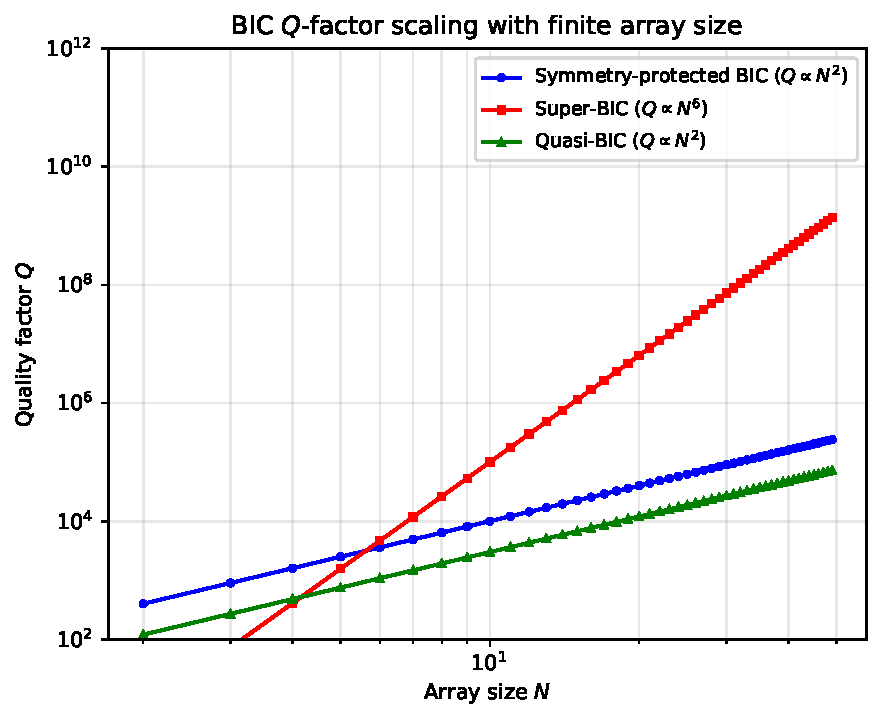
\includegraphics[width=0.6\linewidth]{figures/fig_f16_bic_q_scaling.pdf}
 \caption{Quality-factor scaling with array size $N$ for different BIC
types. A symmetry-protected BIC ($|q| = 1$) and a generic quasi-BIC
both scale as $\Qfac \propto N^2$, while a super-BIC formed by symmetry-
tuned cancellation of lower-order radiation amplitudes can achieve
$\Qfac \propto N^6$, enabling ultralow-threshold lasing in finite
arrays~\cite{hwang2021ultralow}.}
 \label{fig:bic-q-scaling}
\end{figure}

\subsection{Merging charges for steeper suppression}
\label{ssec:merging-charges}

If multiple BICs are brought together by tuning a structural parameter,
their topological charges add, but the finite-size scaling is governed by
which low-order radiation amplitudes are cancelled. Consider a
symmetry-protected BIC at $\Gamma$ with $q_0 = +1$ and accidental BICs
approaching $\Gamma$ along symmetry-related directions. When these
accidental BICs merge with the $\Gamma$-point BIC, symmetry and charge
conservation can cancel not only the leading radiation amplitude but also
the next allowed term. In the super-BIC design of Hwang et al., the
radiation rate near the merged point changes from
$\gamma \propto |\Delta k|^2$ to
\begin{equation}
 \gamma(\Delta k) \propto |\Delta k|^6,
 \label{eq:k6-scaling}
\end{equation}
near the merged point~\cite{hwang2021ultralow}. This sixth-order
suppression is therefore an additional symmetry-tuned cancellation, not
a generic consequence of merely adding two unit charges. In finite arrays
it yields $\Qfac_{\mathrm{finite}} \propto N^6$ instead of $N^2$. The
merged state is called a \emph{super-BIC}.

\begin{figure}[t]
 \centering
 
\includegraphics[width=0.98\textwidth]{fig_f16_q_scaling.pdf}
 \caption{Topological charge engineering changes the quality-factor landscape. Left: an isolated charge-one BIC has radiative loss proportional to $k^2$, hence $Q\propto k^{-2}$, whereas a merged super-BIC can show the much steeper $Q\propto k^{-6}$ scaling discussed in the text. Right: a Brillouin-zone-folding BIC model illustrates the perturbation-controlled scaling $Q\sim 1/(\alpha^2 k^2)$, so reducing the folding perturbation raises the high-$Q$ region over a broad momentum range.}
 \label{fig:bic-q-landscape}
\end{figure}


\subsection{Experimental demonstration: the super-BIC laser}
\label{ssec:super-bic-laser}

Hwang et al.\ demonstrated the super-BIC concept in an InGaAsP photonic
crystal slab laser with a square lattice of air holes and a thickness
of \SI{650}{nm}~\cite{hwang2021ultralow}. By varying the lattice constant
$a$, they traced the evolution through three lasing regimes:

\begin{enumerate}
 \item \textbf{Symmetry-protected BIC laser} ($a < \SI{576.3}{nm}$):
 the mode at $\Gamma$ is a symmetry-protected BIC; the accidental
 BICs sit at finite $|\kk_t|$. The radiation loss follows
 $\gamma \propto [k(k - k_t)(k + k_t)]^2$.

 \item \textbf{Super-BIC laser} ($a \approx \SI{576.3}{nm}$):
 the accidental BICs merge with the $\Gamma$-point BIC. The
   radiation loss becomes $\gamma \propto |\Delta k|^6$, producing the steepest
 suppression and the highest $\Qfac$ in a finite cavity.

 \item \textbf{Post-merging regime} ($a > \SI{576.3}{nm}$):
 only the symmetry-protected BIC remains; the radiation loss
   returns to $\gamma \propto |\Delta k|^2$.
\end{enumerate}

The super-BIC laser achieved a measured threshold of approximately
$\SI{1.47}{kW/cm^2}$ and a quality factor up to $\sim 7300$---with a
threshold power roughly $50$ to $10^7$ times lower than earlier BIC
nanolasers~\cite{hwang2021ultralow}. The far-field image showed strong
angular confinement consistent with the $k^6$ radiation suppression.

\begin{takeaway}[Merging BICs for finite-size performance]
The topological charge framework also functions as a design principle.
By merging BICs with controlled charge, the
radiation scaling near the BIC can be steepened from $k^2$ to $k^6$ or
higher, improving the quality factor of finite-size
photonic cavities. This converts a fundamental limitation of BIC-based
devices (sensitivity to finite size) into an engineering opportunity.
\end{takeaway}


%% ================================================================
\section{Brillouin-zone-folding BICs}
\label{sec:bzf-bic}

An alternative route to high-$\Qfac$ BICs over large momentum-space
regions uses Brillouin zone folding (BZF)~\cite{wang2023brillouin}.

\subsection{Folding guided modes into the continuum}
\label{ssec:bzf-mechanism}

In an unperturbed photonic crystal slab, guided modes below the light
line are perfectly bound---they cannot radiate because their in-plane
wave vector exceeds $\omega/c$. Introducing a periodic perturbation
that doubles the unit cell (e.g., alternating the gap between
neighboring holes or their radii) folds the first Brillouin zone in
half. Guided modes that were at the $X$ or $M$ edge of the original
BZ are folded to the $\Gamma$ point of the new, smaller BZ---placing
them inside the light cone, where radiation channels are open.

Despite now lying within the continuum, these folded modes can remain
non-radiating if the perturbation preserves the conditions for a BIC.
The resulting states are called \emph{Brillouin-zone-folding BICs}
(BZF-BICs).

\subsection{Q-factor scaling and perturbation control}
\label{ssec:bzf-q-scaling}

Unlike conventional BICs, whose $\Qfac$ drops quadratically away from
the BIC point as $\Qfac \propto 1/(k - k_{\mathrm{BIC}})^2$, BZF-BICs
exhibit a perturbation-dependent enhancement of $\Qfac$ across a large
region of momentum space. For a BZF-BIC induced by a perturbation of
strength $\alpha$, the quality factor scales as
\begin{equation}
 \Qfac = \frac{\Qfac_0}{\alpha^2\,k^2},
 \label{eq:bzf-q-scaling}
\end{equation}
where $\Qfac_0$ depends on the unperturbed guided-mode structure.
Reducing $\alpha$ uniformly increases $\Qfac$ across a broad range of
$k$ values, rather than only at the single BIC
point~\cite{wang2023brillouin}.

\subsection{Disorder robustness}
\label{ssec:bzf-disorder}

A major practical advantage of BZF-BICs is their robustness against
fabrication disorder. Wang et al.\ demonstrated that even when
structural disorder is introduced, the $\Qfac$ of BZF-BICs remains at
least ten times higher than that of conventional BICs under the same
disorder level~\cite{wang2023brillouin}. This robustness arises because
the BZF-BIC quality factor is controlled by the perturbation strength
$\alpha$, not by the proximity to a single topological singularity that
can be shifted by disorder.


%% ================================================================
\section{BICs and exceptional points}
\label{sec:bic-ep}

BICs and exceptional points are connected through the analytic structure
of the scattering matrix. Near a BIC, the resonance width $\gamma(\kk)$
vanishes, and two poles of the scattering matrix---the resonance and its
time-reversed partner---approach the real axis. Under perturbation, these
poles can either split into a pair of finite-width resonances or coalesce
into an exceptional point.

\subsection{EP rings around BICs}
\label{ssec:ep-ring}

In certain photonic crystal slabs, perturbing a BIC can produce a ring
or chain of exceptional points in the $(k_x,k_y)$ plane. Inside and
outside such a ring the two relevant resonance sheets have different
real and imaginary splitting patterns, analogous to the unbroken and
broken sectors of a two-mode non-Hermitian model. The EP ring is the
locus where the two resonances coalesce. Its existence is model
dependent; the BIC charge constrains the possible topology but does not
guarantee an EP ring in every slab.

The radius of the EP ring is controlled by the strength of the
perturbation that breaks the BIC condition. As the perturbation
vanishes, the ring contracts to a point---the BIC itself---and the EP
degeneracy is resolved.

\subsection{Merging BICs and EPs}
\label{ssec:bic-ep-merge}

When two BICs of opposite charge are brought together by tuning a
parameter, they can annihilate and leave behind finite-width resonances.
In models where the same tuning also creates an EP, the topology of the
BIC charges is reflected in the EP discriminant number
(Section~\ref{sec:ep-topology}). The simultaneous appearance of an EP is
therefore an important mechanism, not a universal rule.

This BIC--EP connection provides a unified perspective on non-Hermitian
singularities in photonic systems: BICs are real-frequency topological
defects of the radiation field, while EPs are complex-frequency
topological defects of the eigenvalue surface. The two types of
singularity can transform into each other as parameters are varied.

\subsection{Exceptional surfaces from BIC perturbation}
\label{ssec:ep-surface}

In a photonic crystal slab with two tunable parameters---for example the
slab thickness $d$ and the hole radius $r$---each BIC sits at a
specific point $(\kk_{\mathrm{BIC}}, d, r)$ in the combined
parameter-momentum space. As $d$ and $r$ vary, the BIC traces a curve
in this space, and the EP ring surrounding each BIC sweeps out a
two-dimensional \emph{exceptional surface}. This surface separates
regions with different resonance-sheet structure. The topology of the exceptional surface is constrained
by the topological charges of the BICs it encloses. In slab models where
the far-field radiation channels and eigenvalue sheets share a common
branch structure, the enclosed BIC charges determine the allowed topology
of the exceptional surface. This relation is model-dependent rather than
a universal Euler-characteristic theorem, but it provides a useful
organising principle for the design of non-Hermitian photonic devices
that exploit both BICs and EPs.


%% ================================================================
\section{Quasi-BIC resonances and applications}
\label{sec:quasi-bic}

\subsection{Quasi-BICs as high-$\Qfac$ resonances}
\label{ssec:quasi-bic-resonances}

Near a BIC, the quality factor can be made arbitrarily large by
approaching $\kk_{\mathrm{BIC}}$ in momentum space. These
quasi-BIC resonances combine the high field enhancement of a
near-infinite $\Qfac$ with the radiative coupling needed for
input/output---an ideal combination for sensing, lasing, and
nonlinear optics.

The spectral lineshape of a quasi-BIC resonance is a sharp asymmetric
Fano profile, arising from the interference between the narrow resonant
mode and the broad background of the radiation continuum. The Fano
asymmetry parameter $q_{\mathrm{Fano}}$ is directly related to the
radiation amplitudes $c_j$ and can be tuned by structural parameters.

\subsection{BIC lasers}
\label{ssec:bic-lasers}

Photonic crystal slab lasers based on BIC or quasi-BIC modes can achieve
single-mode lasing with high power and narrow linewidth. The topological
charge protects the existence and motion of the radiation zero under
symmetry-preserving perturbations, while the actual lasing threshold and
linewidth remain sensitive to finite size, gain saturation, absorption,
and fabrication disorder.

The super-BIC laser discussed in Section~\ref{ssec:super-bic-laser}
represents the current frontier of BIC-based lasing: by merging
topological charges, the finite-size quality factor is maximized
and the threshold is minimized. The measured threshold of
$\sim\SI{1.47}{kW/cm^2}$ in a cavity of only $15 \times 15$ periods
demonstrates that BIC physics can be harnessed even in wavelength-scale
active devices~\cite{hwang2021ultralow}.

\subsection{Nonlinear and sensing applications}
\label{ssec:bic-applications}

The field enhancement near a quasi-BIC can strongly increase
nonlinear optical processes. Second-harmonic generation, four-wave
mixing, and stimulated Raman scattering have all been enhanced by orders
of magnitude using quasi-BIC metasurfaces.

For sensing, the sharp Fano lineshape of a quasi-BIC provides high
spectral sensitivity: a small change in the refractive index of the
surrounding medium shifts the resonance wavelength by
$\delta\lambda=S\,\delta n$, while the narrow linewidth set by $\Qfac$
improves the resolvability of that shift. This enables detection of
molecular monolayers.

\paragraph{Quantitative sensing example.}
A standard figure of merit for refractive-index sensing with a
quasi-BIC metasurface is
\begin{equation}
 \mathrm{FOM} = \frac{S}{\Delta\lambda} = S \times \frac{\Qfac}{\lambda_0},
 \label{eq:bic-fom}
\end{equation}
where $S = \dd\lambda_0/\dd n$ is the spectral sensitivity in nm/RIU
and $\Delta\lambda = \lambda_0/\Qfac$ is the resonance linewidth.
For a silicon-nitride ($\varepsilon \approx 4$) metasurface operating
near $\lambda_0 = 1550\;\mathrm{nm}$ with $S \approx 400\;\mathrm{nm/RIU}$
and a quasi-BIC quality factor $\Qfac = 5000$, the FOM is approximately
$400 \times 5000/1550 \approx 1290$---more than an order of magnitude
higher than typical surface-plasmon sensors ($\mathrm{FOM} \sim 50$--$100$).
The practical limit on the FOM is set by fabrication imperfections
that break the symmetry protecting the BIC, reducing $\Qfac$ from
the ideal infinite value.

\paragraph{Nonlinear enhancement scaling.}
For a Kerr-type $\chi^{(3)}$ nonlinear process, the conversion
efficiency scales as $|E_{\mathrm{local}}/E_{\mathrm{in}}|^4 \propto
\Qfac^2$ because the field enhancement inside the resonator is
proportional to $\sqrt{\Qfac}$. For second-harmonic generation
($\chi^{(2)}$), the scaling is $\propto \Qfac_\omega \times
\Qfac_{2\omega}$, where both the fundamental and harmonic must
resonate. Quasi-BIC metasurfaces have demonstrated SHG conversion
efficiencies exceeding $10^{-5}$ at pump intensities below
$1\;\mathrm{GW/cm^2}$ in GaAs and LiNbO$_3$ platforms---comparable
to or exceeding conventional nonlinear crystals in the same thickness
but with the added advantage of subwavelength confinement and
engineered angular acceptance. The BIC topology helps organize how the
high-$\Qfac$ condition moves under moderate fabrication disorder, but
the achievable enhancement is still limited by symmetry breaking,
absorption, and finite aperture. Quasi-BIC metasurfaces are therefore a
practical, but not disorder-proof, platform for integrated nonlinear
photonics.

\begin{takeaway}[BICs connect Hermitian and non-Hermitian topology]
Bound states in the continuum are real-frequency modes in an open
(non-Hermitian) system, often protected by symmetry, interference, and
quantized far-field charge in momentum space. They connect the Hermitian
world of real eigenfrequencies to the non-Hermitian world of complex
resonances and exceptional points through the polarization topology of
the far field.
Their annihilation, creation, and merging are governed by charge
conservation, and their engineering---through charge merging,
Friedrich--Wintgen avoided crossings, and
Brillouin zone folding---provides concrete design principles for
high-$\Qfac$ photonic devices with finite size and fabrication tolerance.
The quantitative figures of merit developed in this chapter---the sensing
FOM~\eqref{eq:bic-fom}, the $k^6$ super-BIC scaling~\eqref{eq:k6-scaling},
and the perturbation-controlled BZF
enhancement~\eqref{eq:bzf-q-scaling}---translate topological concepts
into device-level performance metrics.
\end{takeaway}
